\begin{adjustwidth*}{}{-2.25in}
\textbf{{\large Exercises}}
\setlength{\columnsep}{25pt}
\begin{multicols*}{2}
\noindent Terms and Concepts \small
\begin{enumerate}[1)]
\item What are the typical units of work?
\item If a man has a mass of $80$ kg on Earth, will his mass on the moon be bigger, smaller, or the same?
\item If a woman weighs $130$ lb on Earth, will her weight on the moon be bigger, smaller, or the same?
\end{enumerate} 

\noindent {\normalsize Problems} \small

\begin{enumerate}[1),resume]
\item A 100 ft rope, weighing 0.1 lb/ft, hangs over the edge of a tall building.
	\begin{enumerate}
	\item		How much work is done pulling the entire rope to the top of the building?
	\item		How much rope is pulled in when half of the total work is done?
	\end{enumerate}

\item A 50 m rope, with a mass density of 0.2 kg/m, hangs over the edge of a tall building.
	\begin{enumerate}
	\item		How much work is done pulling the entire rope to the top of the building?
	\item		How much work is done pulling in the first 20 m?
	\end{enumerate}

\item A rope of length $\ell$ ft hangs over the edge of tall cliff. (Assume the cliff is taller than the length of the rope.) The rope has a weight density of $d$ lb/ft.
	\begin{enumerate}
	\item		How much work is done pulling the entire rope to the top of the cliff?
	\item		What percentage of the total work is done pulling in the first half of the rope?
	\item		How much rope is pulled in when half of the total work is done?
	\end{enumerate}

\item A 20 m rope with mass density of 0.5 kg/m hangs over the edge of a 10 m building. How much work is done pulling the rope to the top?

\item A crane lifts a 2,000 lb load vertically 30 ft with a 1'' cable weighing 1.68 lb/ft.
	\begin{enumerate}
	\item		How much work is done lifting the cable alone?
	\item		How much work is done lifting the load alone?
	\item		Could one conclude that the work done lifting the cable is negligible compared to the work done lifting the load?
	\end{enumerate}

\item A 100 lb bag of sand is lifted uniformly 120 ft in one minute. Sand leaks from the bag at a rate of 1/4 lb/s. What is the total work done in lifting the bag?

\item A box weighing 2 lb lifts 10 lb of sand vertically 50 ft. A crack in the box allows the sand to leak out such that 9 lb of sand is in the box at the end of the trip. Assume the sand leaked out at a uniform rate. What is the total work done in lifting the box and sand?

\item A force of 1000 lb compresses a spring 3 in. How much work is performed in compressing the spring?

\item A force of 2 N stretches a spring 5 cm. How much work is performed in stretching the spring?

\item A force of 50 lb compresses a spring from 18 in to 12 in. How much work is performed in compressing the spring?

\item A force of 20 lb stretches a spring from 6 in to 8 in. How much work is performed in stretching the spring?

\item A force of 7 N stretches a spring from 11 cm to 21 cm. How much work is performed in stretching the spring?

\item A force of $f$ N stretches a spring $d$ m. How much work is performed in stretching the spring?

\item A 20 lb weight is attached to a spring. The weight rests on the spring, compressing the spring from a natural length of 1 ft to 6 in. 

How much work is done in lifting the box 1.5 ft (i.e, the spring will be stretched 1 ft beyond its natural length)?

\item A 20 lb weight is attached to a spring. The weight rests on the spring, compressing the spring from a natural length of 1 ft to 6 in. 

How much work is done in lifting the box 6 in (i.e, bringing the spring back to its natural length)?

\item A 5 m tall cylindrical tank with radius of 2 m is filled with 3 m of gasoline, with a mass density of 737.22 kg/m$^3$. Compute the total work performed in pumping all the gasoline to the top of the tank.

\item A 6 ft cylindrical tank with a radius of 3 ft is filled with water, which has a weight density of 62.4 lb/ft$^3$. The water is to be pumped to a point 2 ft above the top of the tank.
\begin{enumerate}
\item		How much work is performed in pumping all the water from the tank?
\item		How much work is performed in pumping 3 ft of water from the tank?
\item		At what point is 1/2 of the total work done?
\end{enumerate}

\item A gasoline tanker is filled with gasoline with a weight density of 45.93 lb/ft$^3$. The dispensing valve at the base is jammed shut, forcing the operator to empty the tank via pumping the gas to a point 1 ft above the top of the tank. Assume the tank is a perfect cylinder, 20 ft long with a diameter of 7.5 ft. 

How much work is performed in pumping all the gasoline from the tank?

\end{enumerate}

%------------------------------------------
% END OF EXERCISES ON FIRST PAGE
%------------------------------------------
\end{multicols*}
\end{adjustwidth*}

\clearpage

\begin{adjustwidth*}{}{-2.25in}
\setlength{\columnsep}{25pt}
\begin{multicols*}{2}\small

\begin{enumerate}[1),start=22]

\item A fuel oil storage tank is 10 ft deep with trapezoidal sides, 5 ft at the top and 2 ft at the bottom, and is 15 ft wide (see diagram below). Given that fuel oil weighs 55.46 lb/ft$^3$, find the work performed in pumping all the oil from the tank to a point 3 ft above the top of the tank.

\hfill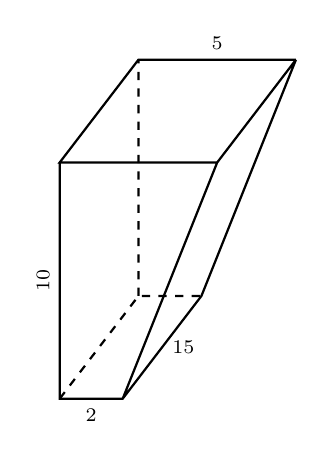
\begin{tikzpicture}[x={(1,0)},z={(0,1)},y={(.5,.87)},xscale=.4,yscale=.3]
\draw [thick] (0,0,0) -- node [above,rotate=90,pos=.5] {\scriptsize 10} (0,0,-10) --  node [below, pos=.5] {\scriptsize 2} (2,0,-10) -- node [right, pos=.5] {\scriptsize 15} (2,5,-10) -- (5,5,0)
							(5,5,0) -- (5,0,0)
							(5,0,0) -- (0,0,0) -- (0,5,0) --  node [above,pos=.5] {\scriptsize 5}(5,5,0)
							(5,0,0) -- (2,0,-10);						

\draw [thick,dashed] (0,0,-10) -- (0,5,-10) -- (2,5,-10)
																	(0,5,-10) -- (0,5,0);
\end{tikzpicture}\hfill\null

\item A conical water tank is 5 m deep with a top radius of 3 m. The tank is filled with pure water, with a mass density of 1000 kg/m$^3$. 
	\begin{enumerate}
	\item		Find the work performed in pumping all the water to the top of the tank.
	\item		Find the work performed in pumping the top 2.5 m of water to the top of the tank.
	\item		Find the work performed in pumping the top half of the water, by volume, to the top of the tank.
	\end{enumerate}

\item A water tank has the shape of a truncated cone, with dimensions given below, and is filled with water with a weight density of 62.4 lb/ft$^3$. Find the work performed in pumping all water to a point 1 ft above the top of the tank.\\

\hfill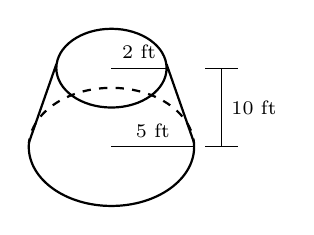
\begin{tikzpicture}[xscale=.7,yscale=.5]\draw [thick] (0,0) circle (1)
							(-1,.1) -- (-1.5,-1.9)
							(1,.1) -- (1.5,-1.9);
\draw (0,0)-- node [above,pos=.5] {\scriptsize 2 ft} (1,0)
			(0,-2) -- node [above,pos=.5] {\scriptsize 5 ft} (1.5,-2)
			(1.7,0) -- (2.3,0)
			(1.7,-2) -- (2.3,-2)
			(2,0) -- node [pos=.5,right] {\scriptsize 10 ft} (2,-2);
\draw [thick] (-1.5,-2) arc (180:360:1.5);
\draw [thick,dashed] (-1.5,-2) arc (180:0:1.5);
\end{tikzpicture}
\hfill\null

\item A water tank has the shape of an inverted pyramid, with dimensions given below, and is filled with water with a mass density of 1000 kg/m$^3$. Find the work performed in pumping all water to a point 5 m above the top of the tank.

\hfill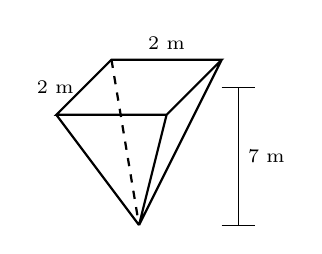
\begin{tikzpicture}[xscale=.7,yscale=.7]
\draw [thick] (0,0) -- node [pos=.5,left]{\scriptsize 2 m} (1,1) --node [above,pos=.5] {\scriptsize 2 m} (3,1) -- (2,0)--cycle
							(0,0) -- (1.5,-2)
							(3,1) -- (1.5,-2)
							(2,0) -- (1.5,-2);
\draw [thick,dashed] (1,1) -- (1.5,-2);
\draw (3,.5) -- (3.6,.5)
			(3,-2) -- (3.6,-2)
			(3.3,.5) -- node [pos=.5,right] {\scriptsize 7 m} (3.3,-2);
\end{tikzpicture}
\hfill\null

\item A water tank has the shape of an truncated, inverted pyramid, with dimensions given below, and is filled with water with a mass density of 1000 kg/m$^3$. Find the work performed in pumping all water to a point 1 m above the top of the tank.

\hfill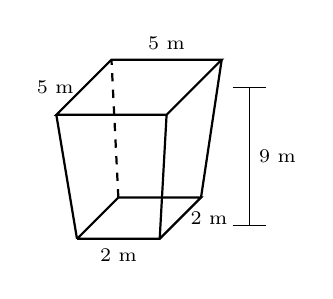
\begin{tikzpicture}[xscale=.7,yscale=.7]
\draw [thick] (0,0) node (A) {}-- node [pos=.5,left]{\scriptsize 5 m} (1,1)node (B) {} --node [above,pos=.5] {\scriptsize 5 m} (3,1) node (C) {} -- (2,0) node (D) {}--cycle;
\begin{scope}[scale=.75,shift={(.5,-3)}]
\draw [thick] (0,0) node (AA) {} -- (1,1) node (BB) {} -- (3,1) node (CC) {} -- node [right,pos=.5] {\scriptsize 2 m} (2,0) node (DD) {}-- node [pos=.5,below]{\scriptsize 2 m} (0,0);
\end{scope}
\draw [dashed,thick] (BB.center) -- (B.center);
\draw [thick] (AA.center) -- (A.center)
							(DD.center) -- (D.center)
							(CC.center) -- (C.center);
\draw (3.2,.5) -- (3.8,.5)
			(3.2,-2) -- (3.8,-2)
			(3.5,.5) -- node [pos=.5,right] {\scriptsize 9 m} (3.5,-2);\end{tikzpicture}
\hfill\null

%\item Consider the curve $f(x) = 3 \cos(\frac{x^3}{4})$ and the portion of its graph that lies in the first quadrant between the $y$-axis and the first positive value of $x$ for which $f(x) = 0$.  Let  $R$ denote the region bounded by this portion of $f$, the $x$-axis, and the $y$-axis.  Assume that $x$ and $y$ are each measured in feet.
%  	\ba
%		\item Picture the coordinate axes rotated 90 degrees clockwise so that the positive $x$-axis points straight down, and the positive $y$-axis points to the right.  Suppose that $R$ is rotated about the $x$ axis to form a solid of revolution, and we consider this solid as a storage tank.  Suppose that the resulting tank is filled to a depth of 1.5 feet with water weighing 62.4 pounds per cubic foot.  Find the amount of work required to lower the water in the tank until it is 0.5 feet deep, by pumping the water to the top of the tank.
%		\item Again picture the coordinate axes rotated 90 degrees clockwise so that the positive $x$-axis points straight down, and the positive $y$-axis points to the right.  Suppose that $R$, together with its reflection across the $x$-axis, forms one end of a storage tank that is 10 feet long.  Suppose that the resulting tank is filled completely with water weighing 62.4 pounds per cubic foot.  Find a formula for a function that tells the amount of work required to lower the water by $h$ feet.
%		\item Suppose that the tank described in (b) is completely filled with water.  Find the total force due to hydrostatic pressure exerted by the water on one end of the tank.
%	\ea 
  
\item A cylindrical tank, buried on its side, has radius 3 feet and length 10 feet.  It is filled completely with water whose weight density is 62.4 lbs/ft$^3$, and the top of the tank is two feet underground.
	\ba
		\item Set up an integral expression that represents the amount of work required to empty the top half of the water in the tank to a truck whose tank lies 4.5 feet above ground.
  
		\item With the tank now only half-full, set up an integral expression that represents the total force due to hydrostatic pressure against one end of the tank.
	\ea

\end{enumerate}

%---------------------------------------------
% END OF EXERCISES ON SECOND PAGE
%---------------------------------------------
\end{multicols*}
\end{adjustwidth*}

\afterexercises